\begin{ex}
 (UFG) A figura a seguir mostra os diversos caminhos que podem ser percorridos entre as cidades A, B, C e D e os valores dos pedágios desses percursos.


\begin{center}    
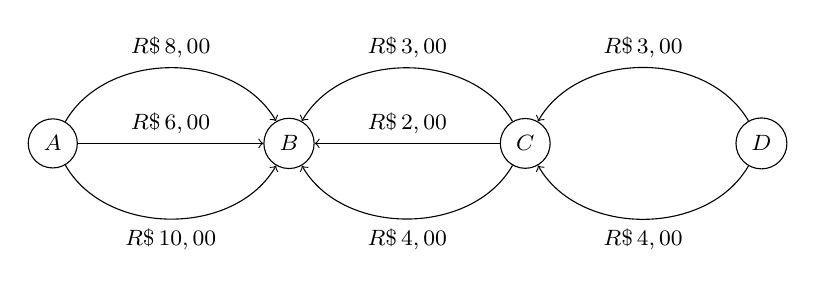
\begin{tikzpicture}

\tikzset{
vertex/.style={circle,draw,minimum size=1em},
edge/.style={->,> = latex'},
font={\fontsize{8pt}{10}\selectfont}
}
% vertices
\node[vertex] (1) at (0,0) {$A$};
\node[vertex] (2) at (3,0) {$B$};
\node[vertex] (3) at (6,0) {$C$};
\node[vertex] (4) at (9,0) {$D$};

%edges
\path[->]
%   FROM       BEND/LOOP      POSIT ION OF LABEL     LABEL      TO
(1) edge[bend left=60]     node[midway, above]   {$R\$\, 8,00$ } (2)
(1) edge[]                 node[midway, above]   {$R\$\, 6,00$ } (2)
(1) edge[bend right=60]    node[midway, below]   {$R\$\, 10,00$} (2)

(3) edge[bend right=60]    node[midway, above]   {$R\$\, 3,00$ } (2)
(3) edge[]                 node[midway, above]   {$R\$\, 2,00$ } (2)
(3) edge[bend left=60]     node[midway, below]   {$R\$\, 4,00$ } (2)

(4) edge[bend right=60]    node[midway, above]   {$R\$\, 3,00$ } (3)
(4) edge[bend left=60]     node[midway, below]   {$R\$\, 4,00$ } (3)

;


% \draw[edge] (1) -- (2) node[midway, above] {$R 6,00$};
% \draw[edge] (1) to[bend left=60] (2) node[midway, above] {$x$};
% \draw[edge] (1) to[bend right=60] (2);

% \draw[edge] (1) -- (3) node[pos=.4, left, sloped, below] {$3$};
% \draw[edge] (1.5) -- (4.145) node[midway, left, sloped, above] {$6$};
% \draw[edge] (2) -- (3) node[pos=.4, left, sloped, above] {$5$};
% \draw[edge] (2.350) -- (4.575) node[midway, sloped, below] {$7$};
% \draw[edge] (3) -- (4) node[pos=.4, sloped, above] {$2$};

\end{tikzpicture}
\end{center}



Dois carros partem das cidades A e D respectivamente, e se encontram na cidade B. Sabendo-se que eles escolhem os caminhos ao acaso, a probabilidade de que ambos gastem a mesma quantia com os pedágios é:
    \begin{enumerate}[(a)]
    \item $\frac{1}{18}$
    \item $\frac{1}{9}$
    \item $\frac{1}{6}$
    \item $\frac{1}{2}$
    \item $\frac{2}{3}$
    \end{enumerate}
      \begin{sol}
        resposta: c \\
        A$\rightarrow$B: carro pode escolher entre 3 caminhos: $\frac{1}{3}$ para cada \\
        D$\rightarrow$B: (3,3) ou (4,2) ou (4,4)= $\frac{1}{2}\cdot\frac{1}{3}+\frac{1}{2}\cdot\frac{1}{3}+\frac{1}{2}\cdot\frac{1}{3}=\frac{1}{2}$\\
        $\Longrightarrow p=\frac{1}{3}\cdot\frac{1}{2}=\frac{1}{6}$
      \end{sol}
\end{ex}